\documentclass[a4paper,11pt]{exam}
\printanswers % pour imprimer les réponses (corrigé)
%\noprintanswers % Pour ne pas imprimer les réponses (énoncé)
\addpoints % Pour compter les points
% \noaddpoints % pour ne pas compter les points
%\qformat{\textbf{\thequestion ) } }
\qformat{\textbf{\thequestion )} (\thepoints) \\} % Pour définir le style des questions (facultatif)
\usepackage{color} % définit une nouvelle couleur
\shadedsolutions % définit le style des réponses
% \framedsolutions % définit le style des réponses
\definecolor{SolutionColor}{rgb}{0.8,0.9,1} % bleu ciel
\renewcommand{\solutiontitle}{\noindent\textbf{Solution:}\par\noindent} % Définit le titre des solutions




\makeatletter

\def\maketitle{{\centering%
	\par{\huge\textbf{\@title}}%
	\par{\@date}%
	\par}}

\makeatother

\lhead{NOM Pr\'enom :}
\rhead{\textbf{Les r\'eponses doivent \^etre justifi\'ees}}
\cfoot{\thepage / \pageref{LastPage}}


%\usepackage{../../pas-math}
%\usepackage{../../moncours}


%\usepackage{pas-cours}
%-------------------------------------------------------------------------------
%          -Packages nécessaires pour écrire en Français et en UTF8-
%-------------------------------------------------------------------------------
\usepackage[utf8]{inputenc}
\usepackage[frenchb]{babel}
\usepackage[T1]{fontenc}
\usepackage{lmodern}
\usepackage{textcomp}



%-------------------------------------------------------------------------------

%-------------------------------------------------------------------------------
%                          -Outils de mise en forme-
%-------------------------------------------------------------------------------
\usepackage{hyperref}
\hypersetup{pdfstartview=XYZ}
%\usepackage{enumerate}
\usepackage{graphicx}
\usepackage{multicol}
\usepackage{tabularx}
\usepackage{multirow}


\usepackage{anysize} %%pour pouvoir mettre les marges qu'on veut
%\marginsize{2.5cm}{2.5cm}{2.5cm}{2.5cm}

\usepackage{indentfirst} %%pour que les premier paragraphes soient aussi indentés
\usepackage{verbatim}
\usepackage{enumitem}
\usepackage[usenames,dvipsnames,svgnames,table]{xcolor}

\usepackage{variations}

%-------------------------------------------------------------------------------


%-------------------------------------------------------------------------------
%                  -Nécessaires pour écrire des mathématiques-
%-------------------------------------------------------------------------------
\usepackage{amsfonts}
\usepackage{amssymb}
\usepackage{amsmath}
\usepackage{amsthm}
\usepackage{tikz}
\usepackage{xlop}
%-------------------------------------------------------------------------------



%-------------------------------------------------------------------------------


%-------------------------------------------------------------------------------
%                    - Mise en forme avancée
%-------------------------------------------------------------------------------

\usepackage{ifthen}
\usepackage{ifmtarg}


\newcommand{\ifTrue}[2]{\ifthenelse{\equal{#1}{true}}{#2}{$\qquad \qquad$}}

%-------------------------------------------------------------------------------

%-------------------------------------------------------------------------------
%                     -Mise en forme d'exercices-
%-------------------------------------------------------------------------------
%\newtheoremstyle{exostyle}
%{\topsep}% espace avant
%{\topsep}% espace apres
%{}% Police utilisee par le style de thm
%{}% Indentation (vide = aucune, \parindent = indentation paragraphe)
%{\bfseries}% Police du titre de thm
%{.}% Signe de ponctuation apres le titre du thm
%{ }% Espace apres le titre du thm (\newline = linebreak)
%{\thmname{#1}\thmnumber{ #2}\thmnote{. \normalfont{\textit{#3}}}}% composants du titre du thm : \thmname = nom du thm, \thmnumber = numéro du thm, \thmnote = sous-titre du thm

%\theoremstyle{exostyle}
%\newtheorem{exercice}{Exercice}
%
%\newenvironment{questions}{
%\begin{enumerate}[\hspace{12pt}\bfseries\itshape a.]}{\end{enumerate}
%} %mettre un 1 à la place du a si on veut des numéros au lieu de lettres pour les questions 
%-------------------------------------------------------------------------------

%-------------------------------------------------------------------------------
%                    - Mise en forme de tableaux -
%-------------------------------------------------------------------------------

\renewcommand{\arraystretch}{1.7}

\setlength{\tabcolsep}{1.2cm}

%-------------------------------------------------------------------------------



%-------------------------------------------------------------------------------
%                    - Racourcis d'écriture -
%-------------------------------------------------------------------------------

% Angles orientés (couples de vecteurs)
\newcommand{\aopp}[2]{(\vec{#1}, \vec{#2})} %Les deuc vecteurs sont positifs
\newcommand{\aopn}[2]{(\vec{#1}, -\vec{#2})} %Le second vecteur est négatif
\newcommand{\aonp}[2]{(-\vec{#1}, \vec{#2})} %Le premier vecteur est négatif
\newcommand{\aonn}[2]{(-\vec{#1}, -\vec{#2})} %Les deux vecteurs sont négatifs

%Ensembles mathématiques
\newcommand{\naturels}{\mathbb{N}} %Nombres naturels
\newcommand{\relatifs}{\mathbb{Z}} %Nombres relatifs
\newcommand{\rationnels}{\mathbb{Q}} %Nombres rationnels
\newcommand{\reels}{\mathbb{R}} %Nombres réels
\newcommand{\complexes}{\mathbb{C}} %Nombres complexes


%Intégration des parenthèses aux cosinus
\newcommand{\cosP}[1]{\cos\left(#1\right)}
\newcommand{\sinP}[1]{\sin\left(#1\right)}


%Probas stats
\newcommand{\stat}{statistique}
\newcommand{\stats}{statistiques}
%-------------------------------------------------------------------------------

%-------------------------------------------------------------------------------
%                    - Mise en page -
%-------------------------------------------------------------------------------

\newcommand{\twoCol}[1]{\begin{multicols}{2}#1\end{multicols}}


\setenumerate[1]{font=\bfseries,label=\textit{\alph*})}
\setenumerate[2]{font=\bfseries,label=\arabic*)}


%-------------------------------------------------------------------------------
%                    - Elements cours -
%-------------------------------------------------------------------------------





%\usepackage{fullpage}
\author{\ }
\date{18 Décembre 2019}
\title{$5^e G$ : DS num\'ero 3}


\begin{document}
%	\usepackage{fancyhdr}
%	
%	\pagestyle{fancy}
%	\fancyhf{}
	%\rhead{Share\LaTeX}

	\maketitle
	
\begin{center}
	\textbf{Calculatrice interdite, toutes les fractions réponse doivent être simplifiées}
\end{center}

\begin{small}
	\begin{center}
		\begin{tabular}{|@{\ }l@{\ }|@{\ }c@{\ }|@{\ }c@{\ }|@{\ }c@{\ }|@{\ }c@{\ }|}
			\hline
			\textbf{Compétence} & \textbf{MI} & \textbf{MF} & \textbf{MS} & \textbf{TBM} \\
			\hline
			\textbf{Représenter} (produire et utiliser plusieurs représentations d’un nombre ) &  \ \ & \ \ & \ \ & \ \  \\
			\hline
			\textbf{Calculer} (calculer avec des nombres rationnels)&  \ \ & \ \ & \ \ & \ \  \\
			\hline	
			\textbf{Raisonne} (résoudre des problèmes impliquant des grandeurs variées) & \ \ & \ \ &  \ \  & \ \ \\
			\hline
%			 
%			\hline
		\end{tabular}
	\end{center}
\end{small}	

	
	
\section{Calculer (2 points)}


\begin{questions}
	\question[1] $\dfrac{1}{4} + \dfrac{5}{2} - \dfrac{3}{4} + 2$
	
	\question[1] $4 - \dfrac{7}{3} - \dfrac{3}{4} + \dfrac{7}{12}$
\end{questions}
	

\section{Le jeu de Lola (3 points bonus)}

Lola propose un jeu à ses deux amis, Juliette et Aurèle.

\begin{center}
	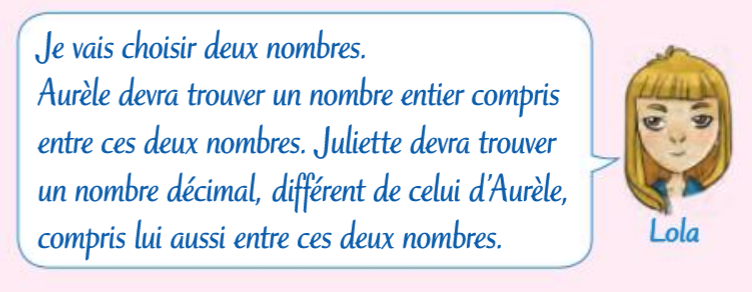
\includegraphics[scale=0.7]{img/lola}
\end{center}

\begin{questions}
	\question[1] Lola a choisi  \num{322.1} et \num{325.4}. Donner toutes les réponses possibles pour Aurèle et dix réponses possibles pour Juliette.
	
	\question[1] Lola choisi tà présent \num{12.3} et \num{12.4}. Donner toutes les réponses possibles pour Aurèle et dix réponses possibles pour Juliette.Peut-on donner toutes les réponses possibles ?
	
	
\question[1] Aurèle n'est pas content et dit à Lola que ses règles du jeu sont injustes. Expliquer pourquoi.
\end{questions}
%\section{Station spatiale (3 points)}

La station spatiale Mir est restée sur orbite pendant 15 ans et a fait à peu près \num{86500} fois le tour de la Terre pendant la durée de son vol spatial.

Le record du plus long séjour dans l'espace revient à Valéri Poliakov qui a vécu 438 jours d'affilée sur Mir.

\begin{questions}
	\question[1\half] Comment faire pour calculer le nombre de fois que ce cosmonaute a fait le tour de la Terre ? (On demande d'expliquer la méthode, pas de faire le calcul.)
	
	
	\question[1\half] \'Ecrire les calculs à faire en une seule expression ? (le résultat n'est pas attendu)
\end{questions}

\section{Voyage (4 points)}

Quatre amis font un voyage en trois jours. Le premier jour, ils parcourent 40 \% du trajet total ; le deuxième jour, un quart et le dernier jour, $\dfrac{7}{20}$ du trajet total.

\begin{questions}
	\question[2] Quel jour ont-ils parcouru la plus grande distance ?
	
	\question[2] Peut-on calculer la distance parcourue chaque jour ?
\end{questions}

\section{Héritage (4 points)}

Après de longues négociations, il a été convenu que Léa héritera de deux quinzièmes de la fortune de son oncle du bout du monde ; Florian, d'un cinquième de cette fortune ; Jean et Justine se partageront équitablement le reste.

\begin{questions}
	\question[2] Quel part de l'héritage sera partagée entre Léa et Florian ?
	\question[2] Quelles seront les parts respectives de Jean et Justine ?
\end{questions}



\section{Une partie de Uno (6 points)}

Quatres copains jouent au Uno. Ce jeu comporte :

\begin{itemize}
	\item des cartes numérotées bleues, rouges, jaunes et vertes (19 de chaque couleur);
	\item 36 cartes Action.
\end{itemize}

\begin{questions}
	\question[2] Quelle proportion du nombre total de cartes représentent les cartes numérotées rouges ?
	\begin{solution}
		$19 \times 4 + 36 = 112$\\
		
		En tout il y a 112 cartes dans le jeu.
		
		Les cartes numérotées rouges représentent $\frac{19}{112}$ du jeu.
	\end{solution}

	
	
	\question[2] Quelle proportion du nombre total de cartes représentent les cartes action ?
	\begin{solution}
		\begin{eqnarray*}
			\dfrac{36}{112} &=& \dfrac{9 \times 4}{28 \times 4} \\
			\dfrac{36}{112} &=& \dfrac{9}{28} \\
		\end{eqnarray*}
	
	Les cartes actions représentent $\frac{9}{28}$ du jeu.
	\end{solution}
	
	\question[2] Au début de la partie, on distribue 7 cartes à chaque joueur et on place le reste dans un paquet au centre de la table. Quelle proportion de cartes n'a pas été distribuée ? Donner le résultat sous forme d'une fraction simplifiée, puis en pourcentage.
	
	\begin{solution}
		Il a quatre joueurs, donc au début de la partie 28 ($7 \times 4$) cartes sont distribuées, il en reste 84.
		
		\begin{eqnarray*}
			\dfrac{84}{112} = \dfrac{3 \times 28}{4 \times 28} \\
			\dfrac{84}{112} = \dfrac{3}{4} \\
		\end{eqnarray*}
	
		Donc $\frac{3}{4}$ des cartes n'ont pas été distribuées, soit 75 \%.
	\end{solution}
\end{questions}

\section{Bonus : Compléter une grille (3 points)}

Chaque ligne et chaque colonne  de la grille ci-dessous doit contenir les quatre même nombres.

%\begin{multicols}{2}
	\begin{questions}
		\question[1] Recopier la grille et remplacer :
		
		\begin{itemize}
			\item A par le numérateur de $\dfrac{19}{3} - 5$,
			\item B par la somme de $\dfrac{1}{6}$, $\dfrac{1}{3}$ et $\dfrac{1}{2}$,
			\item C par le dénominateur de $\dfrac{19}{6}$,
			\item D par $\dfrac{5}{2} + \dfrac{4}{5} + \dfrac{17}{10}$ ,
		\end{itemize}
	
		\begin{solution}
			\begin{eqnarray*}
				\dfrac{19}{3} - 5 = \dfrac{19}{3} - \dfrac{15}{3} \\
				\dfrac{19}{3} - 5 = \dfrac{4}{3}
 			\end{eqnarray*}
 		
 			\begin{eqnarray*}
 				\dfrac{1}{6} + \dfrac{1}{3} + \dfrac{1}{2} = \dfrac{1}{6} + \dfrac{2}{6} + \dfrac{3}{6}\\
 				\dfrac{1}{6} + \dfrac{1}{3} + \dfrac{1}{2} = \dfrac{6}{6} \\
 				\dfrac{1}{6} + \dfrac{1}{3} + \dfrac{1}{2} = 1 \\
 			\end{eqnarray*}
 		
 		
 			\begin{eqnarray*}
 				\dfrac{5}{2} + \dfrac{4}{5} + \dfrac{17}{10} = \dfrac{25}{10} + \dfrac{8}{10} + \dfrac{17}{10}\\
 				\dfrac{5}{2} + \dfrac{4}{5} + \dfrac{17}{10} = \dfrac{50}{10} \\
 				\dfrac{5}{2} + \dfrac{4}{5} + \dfrac{17}{10} = 5 \\
 			\end{eqnarray*}
 		
 		On a donc $A=4$, $B=1$, $C=6$ et $D=5$
		\end{solution}
	
		\question[2] Compléter la grille (Plusieurs réponses sont possibles).
		\begin{solution}
			\begin{center}
				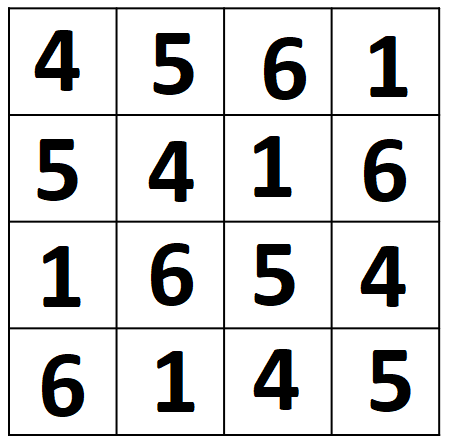
\includegraphics[scale=0.5]{img/grille2}
			\end{center}
		\end{solution}
		
	\end{questions}

	\begin{center}
		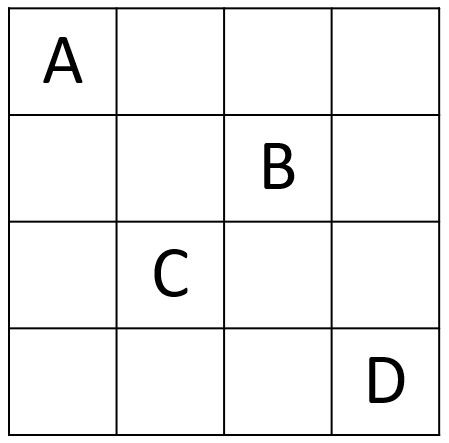
\includegraphics[scale=0.5]{img/grille}
	\end{center}
%\end{multicols}

\label{LastPage}

%\section{Consommation électrique}
%
%Une consommation d'électricité se mesure en 
\end{document}